\chapter{Обучение мультиагентных систем} \label{ch2}


%\section{Введение} \label{ch2:intro}

В этой главе представлена соответствующая работа по теме «Мультиагентное глубокое обучение с подкреплением». Прежде всего, речь идет о современных алгоритмах, которые соответствуют мультиагентным сценариям, выбранным в данной работе.

\section{Мультиагентные алгоритмы} \label{ch2:ma-algs} %название по-русски

Методы обучения с подкреплением, которые специализируются на решении задач с одним агентом, плохо адаптированы для многих реальных задач, таких как автономные транспортные средства, управление водоразделом, согласованный поиск объектов, управление городским траффиком, тороговля на фондовом рынке. Поэтому необходимо расширить эти алгоритмы или даже создать новые для более сложных сценариев с настройками для нескольких агентов.

Некоторые алгоритмы, которые вдохновили эту работу, иллюстрируются в следующих разделах. Этими алгоритмами являются Multi Agent Deep Deterministic Policy Gradient \cite{lowe2017multiagent}, Counterfactual baseline for multi-agent policy gradient \cite{foerster2017counterfactual} и emergent grounded compositional language \cite{mordatch2017emergence}.

\subsection{Детерминированная политика для нескольких агентов}

Multi Agent Deep Deterministic Policy Gradient (\hyperref[acr:maddpg]{MADDPG}) --- это расширение \hyperref[acr:ddpg]{DDPG}, применяемое к настройкам нескольких агентов. Чтобы учесть все состояния среды и политики всех агентов RL в игровом сценарии, алгоритм учитывает совместные наблюдения и действия всех агентов при обучении сетей акторов и критиков. Когда дело доходит до принятия решения, сеть актора каждого агента учитывает только локальные наблюдения. Эта структура централизованного обучения и децентрализованного исполнения позволяет каждому агенту вычислять оптимальную политику по консистентному градиентному сигналу. \cite{lowe2017multiagent}

\begin{figure}[ht!]
    \center
    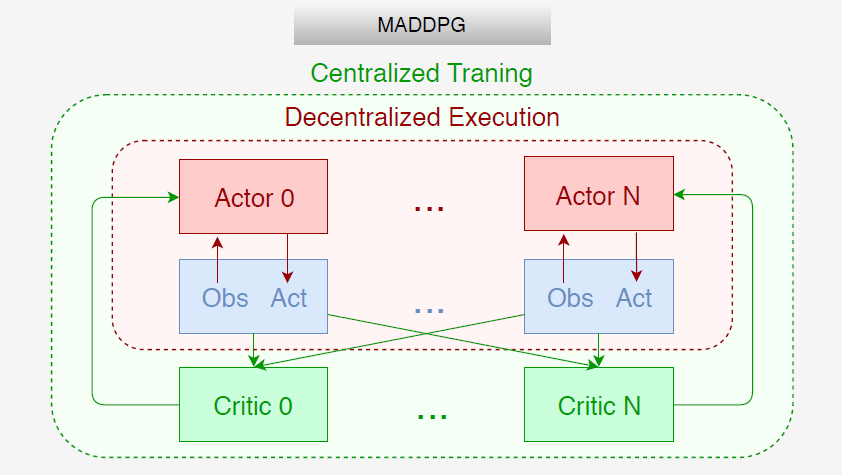
\includegraphics [scale=0.80] {my_folder/images/ch2/maddpg.png}
    \caption{У каждого агента есть децентрализованная сеть акторов, которая получает доступ только к своим локальным наблюдениям. Между тем, каждый агент имеет централизованную сеть критиков, которые имеют доступ к наблюдениям и действиям всех агентов. Критик сети обучен обновлять себя и актора. Основано на \cite{lowe2017multiagent}}
    \label{fig:ch2-maddpg}
\end{figure}

Совместные наблюдения всех агентов обозначаются через $\mathbf{x} = (o_1, ..., o_N)$, совместные действия --- через $a = (a_1, ..., a_N)$. Они вместе с наградами $r$ хранятся в буфере $D$ в виде $(\mathbf{x}, a, r, \mathbf{x}')$. Случайная выборка из $S$ выборок $(\mathbf{x}^j, a^j, r^j, \mathbf{x}'^j)$ извлекается из $D$, а \textit{критик} каждого агента обновляется путём минимизации потерь:

\begin{equation}
    \begin{multlined}
        L(\theta_i) = \dfrac{1}{S} \sum_j (y^j - Q_{i}^\mu (\mathbf x^j, a_{1}^j, ...,a_{N}^j))^2
    \end{multlined}
\end{equation}.

И \textit{актор} обновляется семплированым градиентом политики:

\begin{equation}
    \begin{multlined}
        \nabla_{\theta_i} J \approx \dfrac{1}{S} \sum_j \nabla_{\theta_i} \mu_i (o^j_i) \nabla_{a_i} Q^\mu_i (x^j, a^j_1, ..., a_i, ..., a^j_N)|_{a_i=\mu_i(o^j_i)}
    \end{multlined}
\end{equation}.

Подобно DDPG, целевые сети обновляются «мягко» на каждом шаге на $\theta' \leftarrow \tau \theta + (1 - \tau) \theta'$ с $\tau \ll 1$.

Алгоритм MADDPG хорошо подходит для сценариев с физической навигацией. Было решено продолжить изучение этого алгоритма с помощью многомерного пространства действий, Он хорошо подходит для сценариев, в которых агенты могут взаимодействовать при выполнении физических действий.

\subsection{Контрафактный мультиагентный градиент политики (Counterfactual Multi-Agent Policy Gradient, COMA)}

Контрфактический мультиагентный градиент политики (\hyperref[acr:coma]{COMA}) - это мультиагентный вариант метода \textit{актор-критик}, который использует единого централизованного \textit{критика} для приближения к Q-функции и отдельных децентрализованных \textit{акторов} для оптимизации политики каждого агента $\pi (h)$. \cite{foerster2017counterfactual}

В кооперативных задачах с несколькими агентами сложность сотрудничества возрастает с увеличением количества агентов. Таким образом, было бы нецелесообразно и неэффективно иметь одну единственную оптимальную политику для всех агентов. Вместо этого децентрализованные политики для каждого агента формулируются в виде проблем с несколькими агентами. В COMA один централизованный критик и отдельные акторы тренируются на совместных действиях и совместных наблюдениях. Когда дело доходит до исполнения, каждый актор генерирует действия на основе собственной истории наблюдения $h$, см. \firef{fig:ch2-coma}.

\begin{figure}[ht!]
    \center
    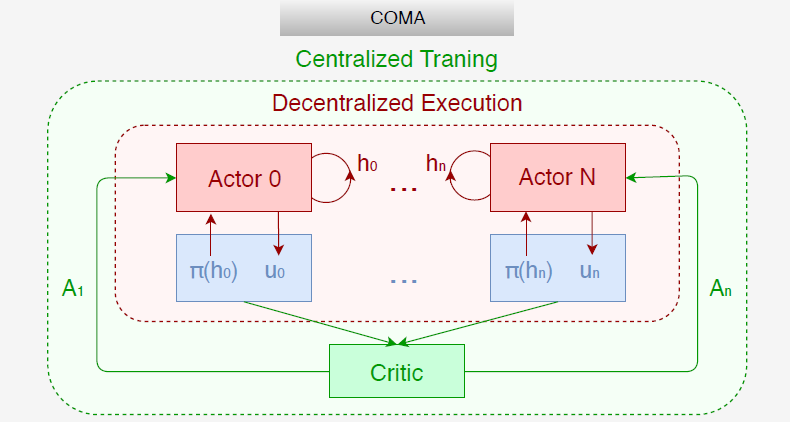
\includegraphics [scale=0.80] {my_folder/images/ch2/coma.png}
    \caption{Структура сетей алгоритма COMA и информационный поток между централизованным критиком и децентрализованными акторами. В COMA отдельно происходит обучение одного централизованного критика и каждого из акторов. Каждый актор децентрализован, при принятии решений использует локальную историю наблюдения $h$ \cite{foerster2017counterfactual}}
    \label{fig:ch2-coma}
\end{figure}

COMA предназначен для мультиагентных совместных сценариев с глобальной функцией награды для всех агентов. Однако агенты, обученные COMA, изучают отдельные политики без явного общения. \cite{foerster2017counterfactual}

\subsection{Возникающий язык (Emergent Language)}

Grounded compositional language обозначает простой язык, где агенты связывают конкретные символы с конкретными объектами, а затем объединяют эти символы в значимые понятия \cite{Szabo2008-SZAC}. Язык представлен в виде абстрактных дискретных символов, произнесённых агентами, которые не имеют заранее определённого значения, но возникли и сформировались в процессе обучения в соответствии со средой и целями \cite{mordatch2017emergence}. В отличие от естественного языка, для работы с которым извлекаются языковые шаблоны из большого набора текстовых данных, этот язык, возникший во время обучения с подкреплением, понятен только агентам и используется ими для сотрудничества друг с другом в достижении общих целей.

\section{Действия и награды} \label{ch2:act-rew} %название по-русски

\subsection{Архитектура ветвления действий (Action Branching)}

Обычно довольно трудно исследовать проблемы с многомерными пространствами действий. Архитектура \textit{ветвления действий} предназначена для решения таких проблем. Например, в среде с \textit{N}-мерным пространством действий и $d_n$ дискретных последующих действий для каждого измерения \textit{n} необходимо рассмотреть в общей сложности $\Pi^N_{n=1} d_n$ возможных действий \cite{tavakoli2017action}. Правильно спроектированные разветвленные архитектуры действий могут эффективно и результативно исследовать такое большое многомерное пространство действий \cite{tavakoli2017action}.

\begin{figure}[ht!]
    \center
    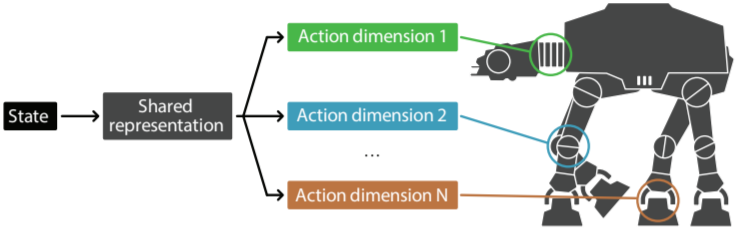
\includegraphics [scale=0.80] {my_folder/images/ch2/action-branching.png}
    \caption{Архитектура сети для ветвления действий, например, для робота, где сеть принимает состояние в качестве входных данных и разделяет нижние уровни для извлечения представлений признаков, а затем расходится по ветвям для относительно независимых под-действий, включая, например, высказывание, действие рукой, действие ногой и т. д. Основано на \cite{tavakoli2017action}.}
    \label{fig:ch2-action-branching}
\end{figure} % TODO: перевести

Основной идеей архитектуры является модуль совместного принятия решений, который извлекает скрытое представление из входного наблюдения и создает отдельные выходные ветви для каждого измерения действия. На рисунке \firef{fig:ch2-action-branching} представлена архитектура \textit{ветвления действий}. \textit{n} измерений действий представляют собой \textit{n} относительно независимых под-действий.
В архитектурах \textit{ветвления действий} значения \textit{Q} рассчитываются для каждого измерения действия. Тем не менее, мы бы хотели, чтобы многомерное действие оценивало одно единственное \textit{Q}-значение, выводимое сетью критика.

\subsection{Архитектура гибридного вознаграждения} % TODO: "Декомпозированная награда"?

Как показано в \cite{seijen2017hybrid}, жизненно важно иметь точную оптимальную value-функцию в обучении с подкреплением, поскольку она оценивает ожидаемый return как сигнал для оптимизации политики. Как только оптимальная value-функция изучена, из неё можно получить оптимальную политику.

\begin{figure}[ht!]
    \center
    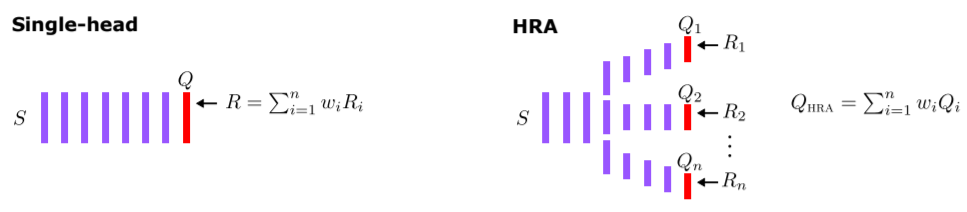
\includegraphics [scale=0.80] {my_folder/images/ch2/hybrid-reward.png}
    \caption{Глубокая нейронная сеть с одной головой, аппроксимирует одну единственную Q-функцию с глобальной функцией награды (слева), и Q-сеть с гибридной архитектурой вознаграждения (справа). Сеть имеет n голов, аппроксимирующих n Q-функций. Каждая Q-функция оценивает Q-значение с помощью соответствующей разложенной функции награды. Основано на \cite{seijen2017hybrid}.}
    \label{fig:ch2-hybrid-reward}
\end{figure} % TODO: перевести

Более того, две разные value-функции могут привести к одной и той же политике, когда агент действует жадно в соответствии с ними \cite{seijen2017hybrid}. Следовательно, можно было бы изучить несколько более простых value-функций, если изучить сложную value-функцию сложно или даже невозможно. В таком случае глобальная функция награды может быть соответственно разложена на несколько различных функций награды:

\begin{equation}
    \begin{multlined}
        R_{rev}(s, a, s') = \sum^n_{k=1} R_k (s, a, s')
    \end{multlined}
\end{equation}

где $R_{rev}$ - глобальная функция награды, которая разбита на \textit{n} функций награды. Каждая разложенная функция награды зависит от подмножества состояний и имеет свою собственную функцию \textit{Q}-значения. Глубокая \textit{Q}-сеть с общими нижними слоями и \textit{n} головами используется для аппроксимации \textit{n} \textit{Q}-значений, обусловливающих текущее состояние и действие с различными функциями разложения награды \firef{fig:ch2-hybrid-reward}.

\begin{equation}
    \begin{multlined}
        Q_{H R A}(s, a; \theta) := \sum^n_{k=1} Q_k(s, a;\theta)
    \end{multlined}
\end{equation}

Q-сеть затем итеративно улучшается за счет оптимизации функции потерь

\begin{equation}
    \begin{multlined}
        L_i(\theta_i) = \mathbb{E}_{s, a, r, s'}[\sum^n_{k=1}(y_{k, i}-Q_k(s, a;\theta_i))^2]
    \end{multlined}
\end{equation}

где

\begin{equation}
    \begin{multlined}
        y_{k, i} = R_k(s, a, s') + \gamma \max_{a'} Q_k(s', a';\theta_{i-1})
    \end{multlined}
\end{equation}

$\theta_i$ — это веса Q-сети в текущей итерации \textit{i}, а $\theta_{i-1}$ - веса отдельной целевой сети в предыдущей итерации.
В гибридной архитектуре вознаграждений \textit{n} \textit{Q}-значений выводятся \textit{n} головами из одной единственной \textit{Q}-сети. Однако для того, чтобы иметь консистентный градиент для улучшения политики для каждого измерения действий, следует создавать отдельные \textit{Q}-сети для оценки \textit{Q}-значений для каждого измерения действий.



\section{Учебная программа}

Обучение по учебной программе — это стратегия обучения, основанная на процессе обучения человека. В системе образования люди обучаются путём ознакомления с концепциями, которые строятся от простых до сложных уровней, от конкретных до более абстрактных уровней, от простых структур до сложных модулей.

Машинное обучение заимствует такой подход. Учебная программа усложняет обучение программы от небольших подзадач или простых аспектов к более тяжёлым и сложным задачам. Ожидается, что обученная модель достигнет высокой эффективности и результатов обучения \cite{10.5555/3171837.3172051}.

В методе учебная программа простой аспект проблемы проливает свет на общую картину, а сложные факторы постепенно добавляются и раскрывают больше деталей целой картины. Поиск решения для сглаженной версии проблемы и затем переход к более детализированной может помочь обучению решить проблему постепенно \cite{graves2017automated}.

Математически $C_\gamma (\theta)$ определяется как функции стоимости задачи, в которой $\gamma$ - уровень сложности, а $\theta$ - параметры. Начальную сглаженную версию $C_0$ обычно легко оптимизировать, доведя $\theta$ до локального минимума. Локальный минимум затем используется в качестве основы для следующего уровня сложности. С увеличением $\gamma$ $C_\gamma$ становится менее сглаженной при дальнейшем поиске следующего локального минимума на основе предыдущего локального минимума. \cite{10.1145/1553374.1553380}

Учебный план также можно рассматривать как последовательное перевзвешивание, сначала на наборах данных из простых примеров, а затем на полном наборе данных. С увеличением уровня сложности в набор обучающих данных добавляются немного более сложные примеры, которые используются для повторного взвешивания распределения. В конце используется полный набор обучающих данных. \cite{10.1145/1553374.1553380}

\section{Выводы}

Произведённого обзора должно быть достаточно для того, чтобы определиться с применяемыми в данной работе методами. В следующей главе речь пойдёт о них.

\newpage % принудительное начало с новой страницы, использовать только в конце раздела
